% ------------------------------------------------------------------------------
% TYPO3 CMS 8.5 - What's New - Chapter "Backend User Interface" (Dutch Version)
%
% @author	Michael Schams <schams.net>
% @license	Creative Commons BY-NC-SA 3.0
% @link		http://typo3.org/download/release-notes/whats-new/
% @language	English
% ------------------------------------------------------------------------------
% LTXE-CHAPTER-UID:		07b25346-95b1df21-a6ebe09a-49f53f41
% LTXE-CHAPTER-NAME:	Backend User Interface
% ------------------------------------------------------------------------------

\section{Gebruikersinterface backend}
\begin{frame}[fragile]
	\frametitle{Gebruikersinterface backend}

	\begin{center}\huge{Hoofdstuk 1:}\end{center}
	\begin{center}\huge{\color{typo3darkgrey}\textbf{Gebruikersinterface backend}}\end{center}

\end{frame}

% ------------------------------------------------------------------------------
% LTXE-SLIDE-START
% LTXE-SLIDE-UID:		7a857cd6-45a287e5-1dcab4ca-69790231
% LTXE-SLIDE-ORIGIN:	e00709d6-ccb8a4d0-1cca1d28-431a00a5 English
% LTXE-SLIDE-TITLE:		#77910: New Form Framework (1)
% ------------------------------------------------------------------------------
\begin{frame}[fragile]
	\frametitle{Gebruikersinterface backend}
	\framesubtitle{Nieuw raamwerk voor formulieren (1)}

	\begin{itemize}
		\item Er is een nieuw, flexibel raamwerk voor het bouwen van formulieren in TYPO3 CMS 8.5
		\item Het vervangt de oude \textit{Formulierenassistent} gebaseerd op ExtJS en het bijbehorende systeem voor de frontend
		\item De nieuwe \textit{formuliereditor} gebruikt jQuery en heeft een moderne architectuur,
			die zorgt voor flexibiliteit en uitbreidbaarheid
		\item Enorm aanpasbaar en configuratie wordt opgeslagen in YAML-bestanden
		\item De lijst features is indrukwekkend\newline
			\small(complete documentatie volgt later)\normalsize
		\item Video met demonstratie is beschikbaar op YouTube:\newline
			\url{https://www.youtube.com/watch?v=F9sTAOEcTI0}
	\end{itemize}

\end{frame}
% ------------------------------------------------------------------------------
% LTXE-SLIDE-START
% LTXE-SLIDE-UID:		c473b224-bbbd4ac3-d445a70a-f653b3a6
% LTXE-SLIDE-ORIGIN:	3bbca669-629eab1c-0230fd06-71e7071c English
% LTXE-SLIDE-TITLE:		#77910: New Form Framework (2)
% ------------------------------------------------------------------------------
\begin{frame}[fragile]
	\frametitle{Gebruikersinterface backend}
	\framesubtitle{Nieuw raamwerk voor formulieren (2)}

	\begin{figure}
		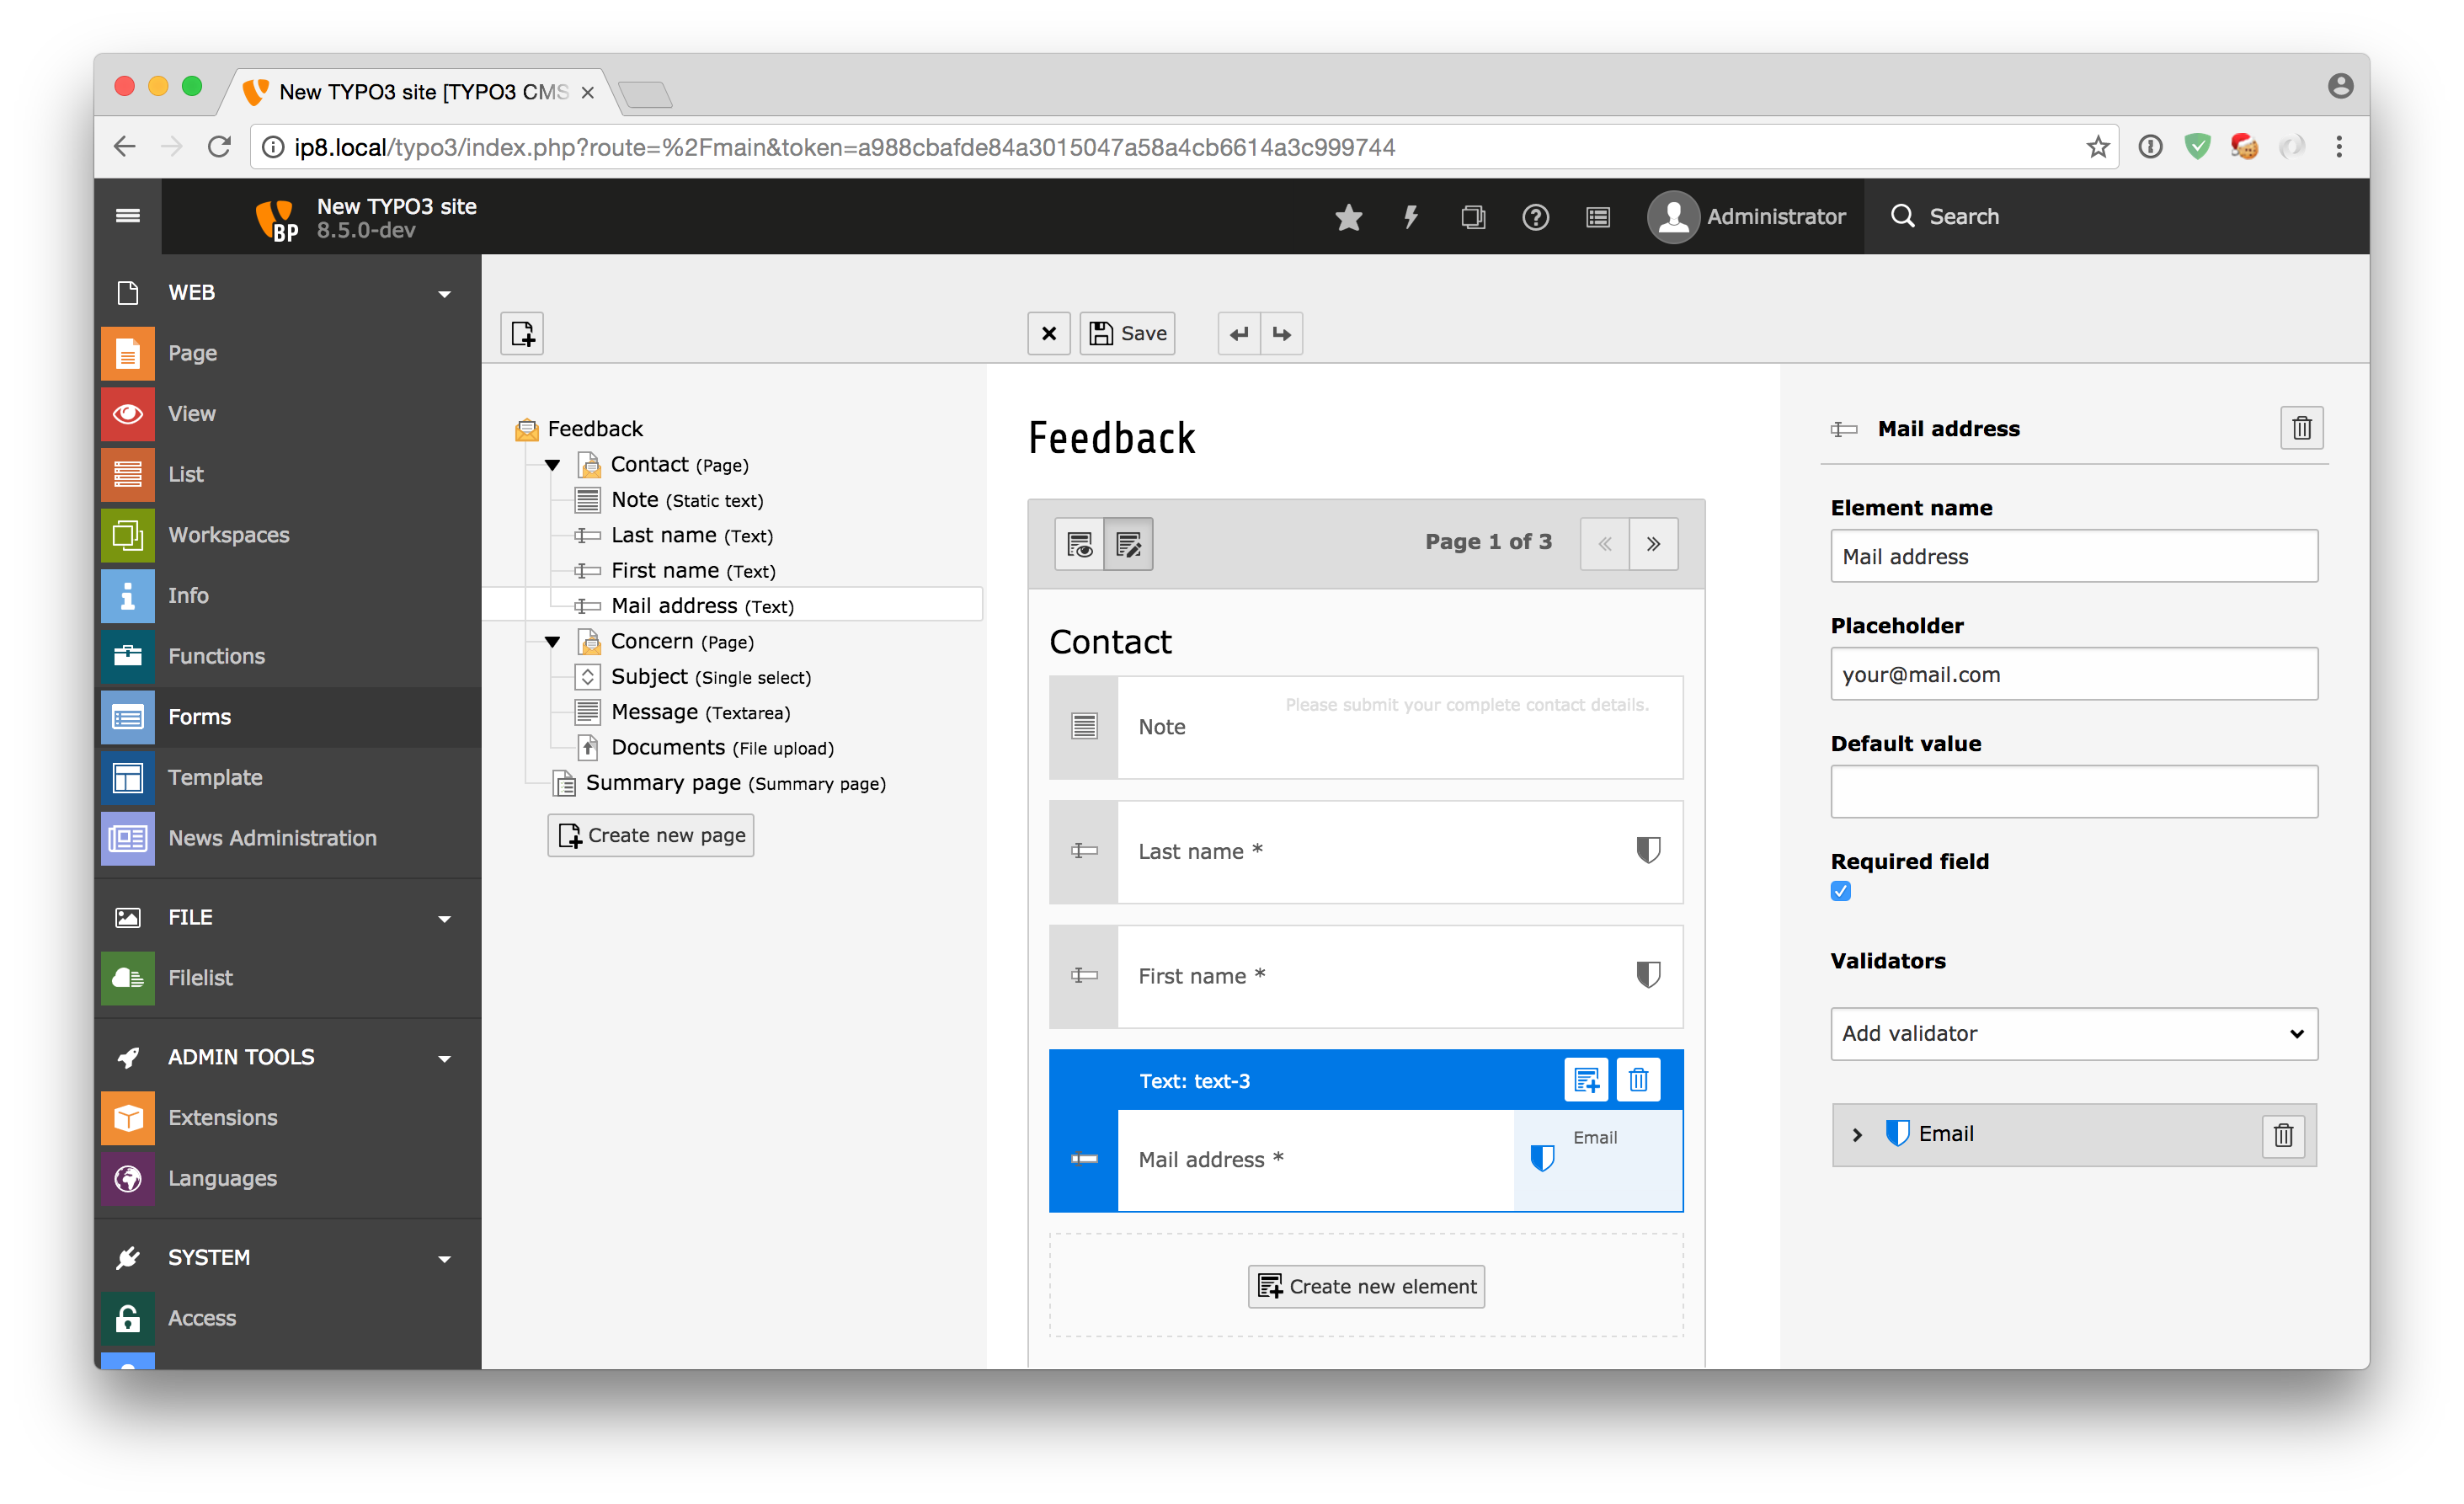
\includegraphics[width=0.8\linewidth]{BackendUserInterface/form-framework-1.png}
	\end{figure}

\end{frame}

% ------------------------------------------------------------------------------
% LTXE-SLIDE-START
% LTXE-SLIDE-UID:		ccca1361-349c7dda-1ac45a30-c3e634eb
% LTXE-SLIDE-ORIGIN:	b91ec75b-7aa7b566-b523ca5f-f9ba3cde English
% LTXE-SLIDE-TITLE:		#77910: New Form Framework (3)
% ------------------------------------------------------------------------------
\begin{frame}[fragile]
	\frametitle{Gebruikersinterface backend}
	\framesubtitle{Nieuw raamwerk voor formulieren (3)}

	\begin{figure}
		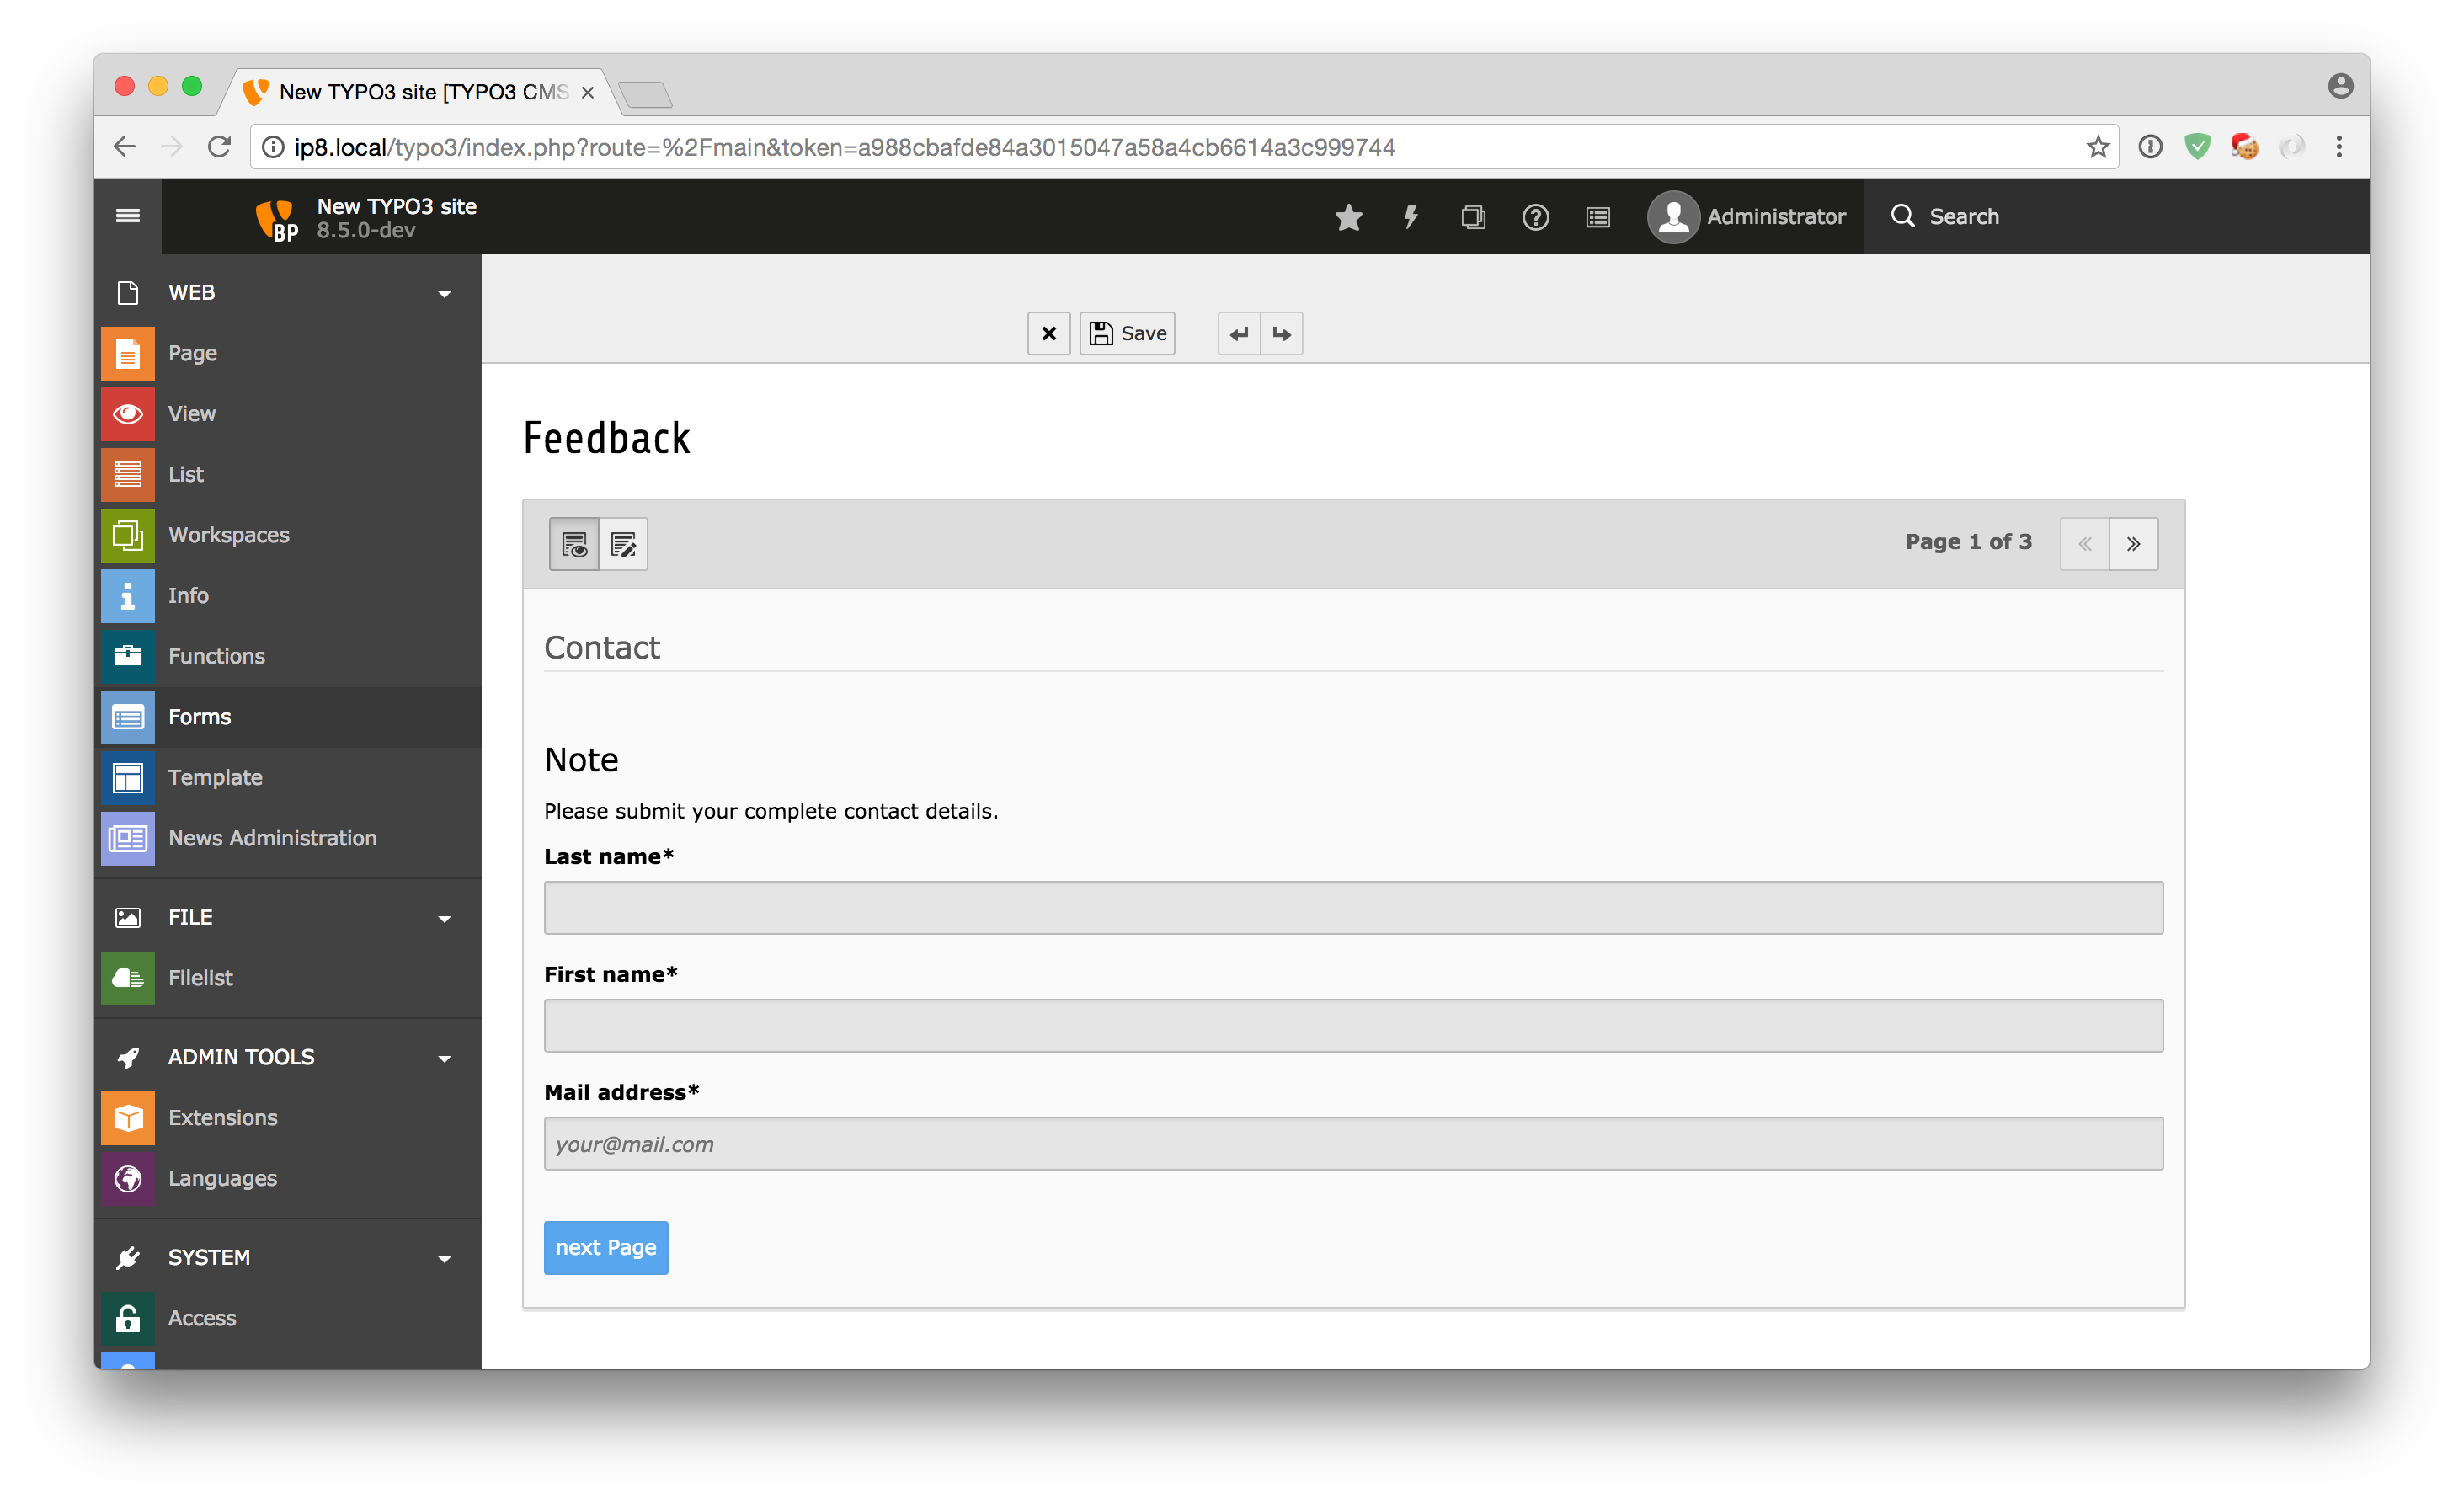
\includegraphics[width=0.8\linewidth]{BackendUserInterface/form-framework-2.png}
	\end{figure}

\end{frame}


% ------------------------------------------------------------------------------
% LTXE-SLIDE-START
% LTXE-SLIDE-UID:		e31b0ab7-5c1b9050-e29a443d-988dc33c
% LTXE-SLIDE-ORIGIN:	c41b2f21-fb92bb80-56e7ddc9-1c725e34 English
% LTXE-SLIDE-TITLE:		CKEditor Integration
% ------------------------------------------------------------------------------
\begin{frame}[fragile]
	\frametitle{Gebruikersinterface backend}
	\framesubtitle{Integratie CKEditor}

	\begin{columns}[T]
		\begin{column}{.5\textwidth}
			De nieuwe generatie tekstverwerking is opgenomen in de TYPO3 backend:
			\textbf{CKEditor}.\newline

			De huidige staat is expliciet aangeduid als \textit{experimenteel} en de extensie
			wordt niet standaard geïnstalleerd.\newline

			Meer details over deze open source tekstverwerker: \url{http://ckeditor.com}
		\end{column}
		\begin{column}{.5\textwidth}
			\begin{figure}\vspace*{-0.4cm}
				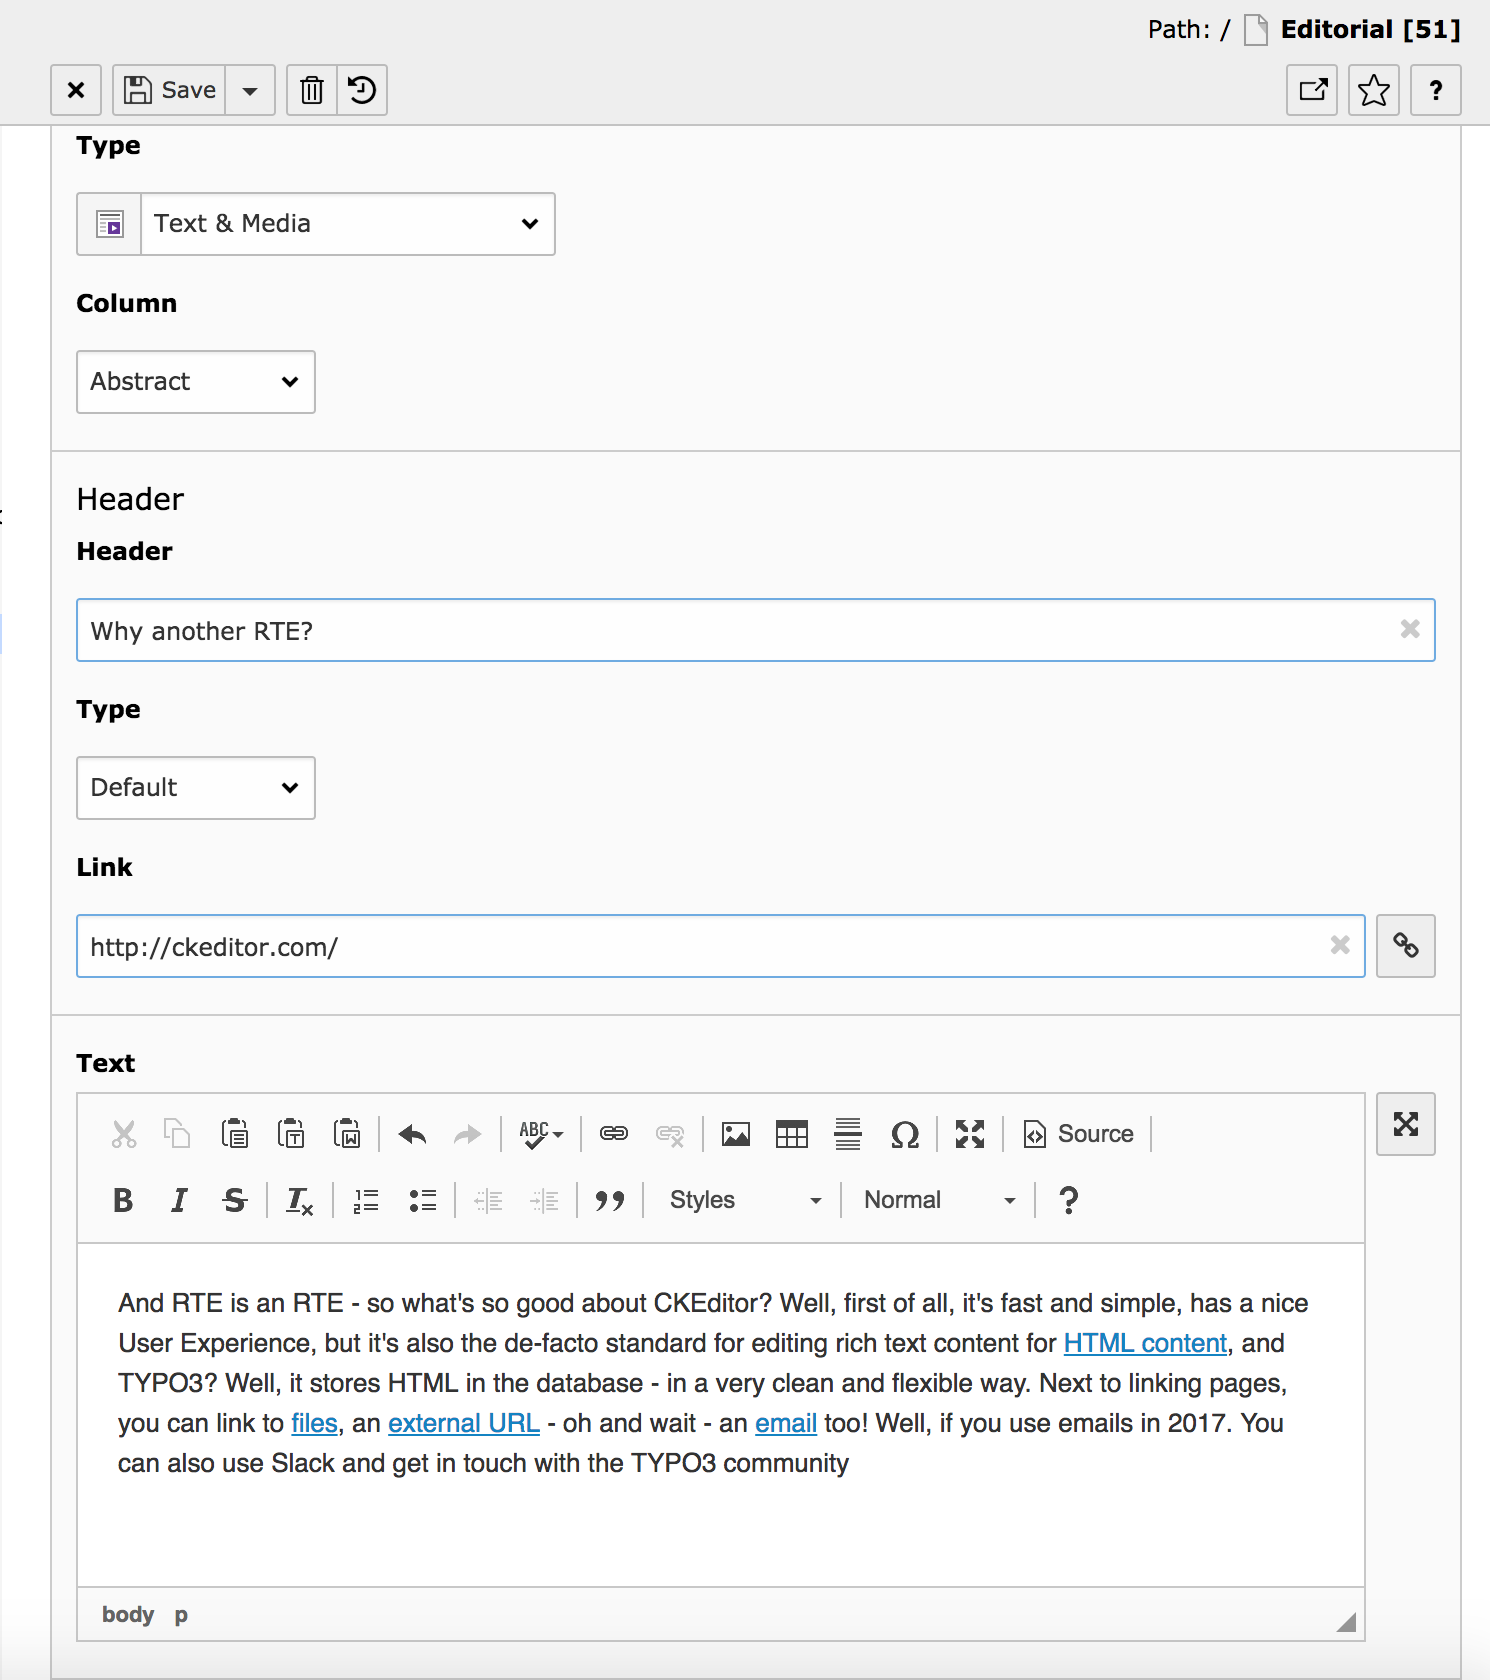
\includegraphics[width=0.8\linewidth]{BackendUserInterface/ckeditor.png}
			\end{figure}
		\end{column}
	\end{columns}

\end{frame}



% ------------------------------------------------------------------------------
% LTXE-SLIDE-START
% LTXE-SLIDE-UID:		cbe69b23-77a1f103-f3ad10d6-44d14c8c
% LTXE-SLIDE-ORIGIN:	c9dc360d-cf218f95-03f53731-03d821ad English
% LTXE-SLIDE-TITLE:		#78383: Field positions in tabs streamlined (TCA)
% ------------------------------------------------------------------------------
\begin{frame}[fragile]
	\frametitle{Gebruikersinterface backend}
	\framesubtitle{Positie en volgorde van elementen}

	\begin{itemize}
		\item De volgorde en positie van bepaalde velden in de TYPO3 backend is verbeterd
		\item Het doel is om tegemoet te komen aan de verwachting van de redacteur waar gebruikelijke opties te vinden zijn
		\item Dit is vooral belangrijk voor vaak gebruikte velden en algemene categorieën die door veel records gedeeld worden
		\item Auteurs van extensies wordt aangemoedigd om de specifieke posities en volgorde van elementen in
			de \href{https://docs.typo3.org}{officiële documentatie} te volgen

			% TODO: update link above (waiting for Doc and Core Team to finish documentation)

	\end{itemize}

	\begin{itemize}
		\item \textit{Een consistente backend is goud waard!} :-)
	\end{itemize}

\end{frame}

% ------------------------------------------------------------------------------
